\subsubsection{Reinforcement Learning}

While Proportional-Integral-Derivative (PID) controllers are the industry standard for stable piloting—offering a simple, "white-box" solution—they often struggle with complex, non-linear dynamics where the Integral term alone is insufficient. Recently, Reinforcement Learning (RL) has gained traction as a robust "black-box" alternative. To reduce the computational burden on onboard systems, reinforcement learning has increasingly been adopted as a key approach for autonomous obstacle avoidance (Yu et al., 2025).

While many RL solutions bridge the gap from computer vision to control, this chapter explores a "target-to-target" approach. Using Unity’s ML-Agents toolkit, I aim to develop a training pipeline that investigates the efficacy of RL for precise drone hovering.

\subsection{Fundamentals of Reinforcement Learning}

The concept of implementing RL in computing is among the earliest visions of AI. In a 1948 report, Alan Turing described a design for a pleasure-pain system (Barto, 2019). Modern RL defines a framework where an agent learns behavior through trial-and-error interactions with a dynamic environment (Kaelbling et al., 1996). Unlike supervised learning, the agent is not provided with "correct" answers. Instead, it receives a scalar reinforcement signal (reward or punishment) and must discover actions that maximize its long-term cumulative reward.

\subsubsection{Markov Decision Processes (MDPs)}

MDPs provide the mathematical foundation for RL \cref{fig:des}. In an MDP, an agent’s actions influence both the immediate reward and the subsequent state of the environment. An MDP is formally defined by:

\begin{itemize}
    \item A set of states (S): Possible environment configurations.
    \item A set of actions (A): Choices available to the agent.
    \item A reward function (R): $R: S \times A \to \mathbb{R}$, specifying the instantaneous reward.
    \item A state transition function (T): $T: S \times A \to \Delta(S)$, defining the probability of transitioning to state $s'$ given action $a$ in state $s$.
\end{itemize}

\begin{figure}
    \caption{Markov Decision Process diagram}
    \label{fig:des}
    \centering
    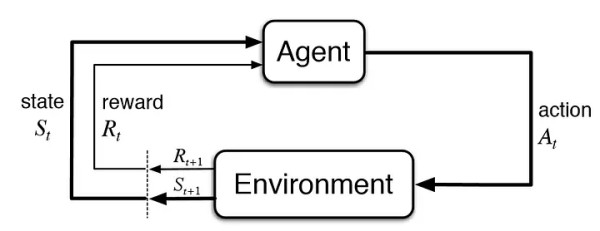
\includegraphics[width=0.8\linewidth]{img/decision.jpg}
\end{figure}